\documentclass[professionalfont]{beamer}
\usepackage{newtxtext}
\usepackage[UTF8, heading = false, scheme = plain]{ctex}
\mode<presentation>{\usetheme{Warsaw}}

\setbeamertemplate{footline}[frame number]
\setbeamertemplate{caption}[numbered]
\usepackage{bbm}
\usepackage{multirow}
\usepackage{amsmath}
\usepackage{listings}
\usepackage{xcolor}
\lstset{basicstyle=\tiny\ttfamily,
	numbers=left,
	escapeinside=||
}
\newcommand{\R}[1]{\textcolor{blue}{\small \textrm{#1}}}
\newcommand{\Rout}[1]{\textcolor{green}{\small \textrm{#1}}}
\newcommand{\red}[1]{\textcolor{red}{#1}}
\newcommand{\green}[1]{\textbf{#1}}
\newcommand{\purple}[1]{\textcolor{purple}{#1}}
\newcommand{\blue}[1]{\textcolor{blue}{#1}}
\newcommand{\gray}[1]{\textcolor{gray}{#1}}
\setbeamertemplate{bibliography item}{\insertbiblabel}
\setbeamercolor{bibliography entry author}{fg=black}
\setbeamercolor{bibliography entry title}{fg=black} 
\setbeamercolor{bibliography entry location}{fg=black} 
\setbeamercolor{bibliography entry note}{fg=black}  

\title{第1讲:非寿险精算简介}
\author{高光远}
\institute{中国人民大学~统计学院}
\date{}
\begin{document}
%%title frame
\begin{frame}
	\titlepage
\end{frame}

%\begin{frame}{主要内容}
%	\tableofcontents
%\end{frame}

%%table of contents
%\AtBeginSection[]
%{
%	\begin{frame}{}
%		\tableofcontents[currentsection]
%	\end{frame}
%}

\begin{frame}{非寿险在全球}
\blue{Non-life insurance} in Continental Europe is also known as \blue{property and casualty insurance (P\&C)} in the US and Canada, and \blue{general insurance} in the UK and Australia. 
\end{frame}

\begin{frame}{精算师协会}
\begin{itemize}
\item \blue{The China Association of Actuaries (CAA)}.
\item \blue{The Casualty Actuarial Society (CAS)} is a North American based actuarial association, specialized in non-life insurance.
\item \blue{The Society of Actuaries (SOA)} is a North American based actuarial association, providing various tracks such as life and annuity, retirement, quantitative finance, general insurance, etc.  
\begin{figure}
\centering

\includegraphics[height=0.1\linewidth]{Plots/caa.jpg}~~

\includegraphics[height=0.1\linewidth]{Plots/logo.png}~~

\includegraphics[height=0.1\linewidth]{Plots/soa.png}
\end{figure}
\item \blue{The Institute and Faculty of Actuaries (IFoA)} is the British actuarial association.
\item \blue{The Institute of Actuaries of Australia (IAA)}.
\end{itemize}
\end{frame}

%\begin{frame}{人大统计学院}
%\begin{figure}
%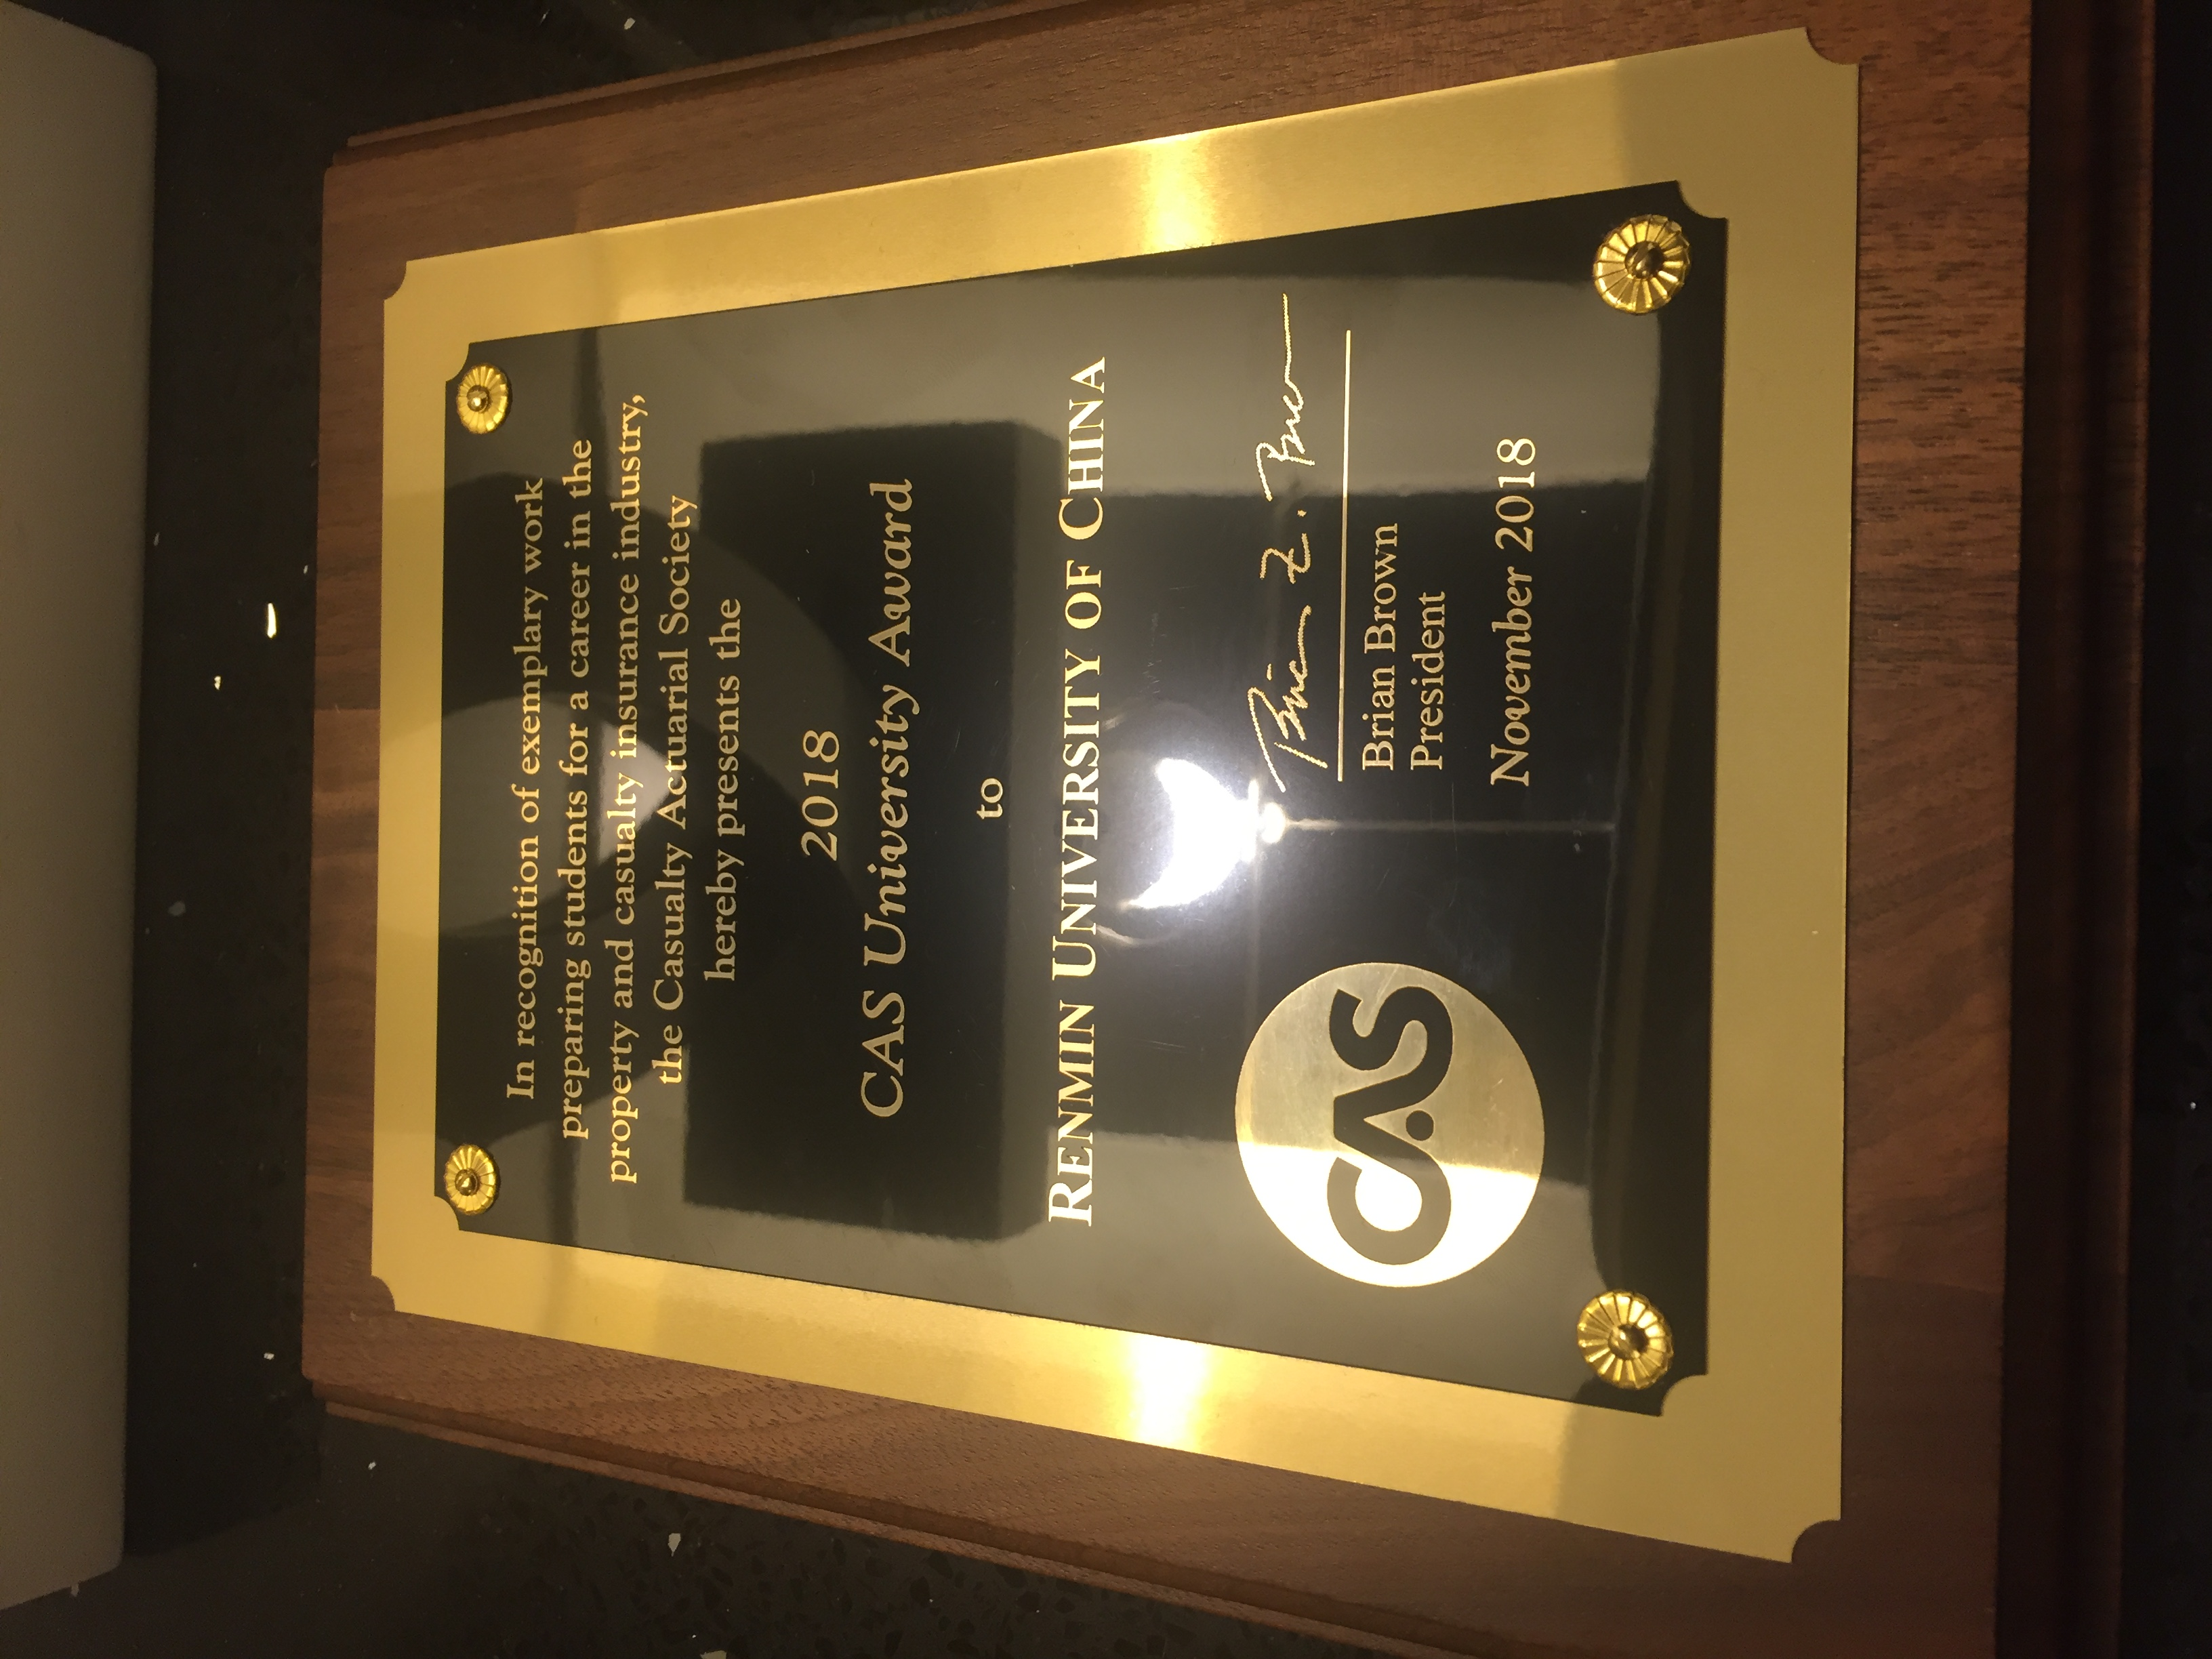
\includegraphics[height=0.5\linewidth, angle=-90]{Plots/cas_award.jpg}
%\end{figure}
%\end{frame}

\begin{frame}{1666年伦敦大火}
\begin{figure}
\centering
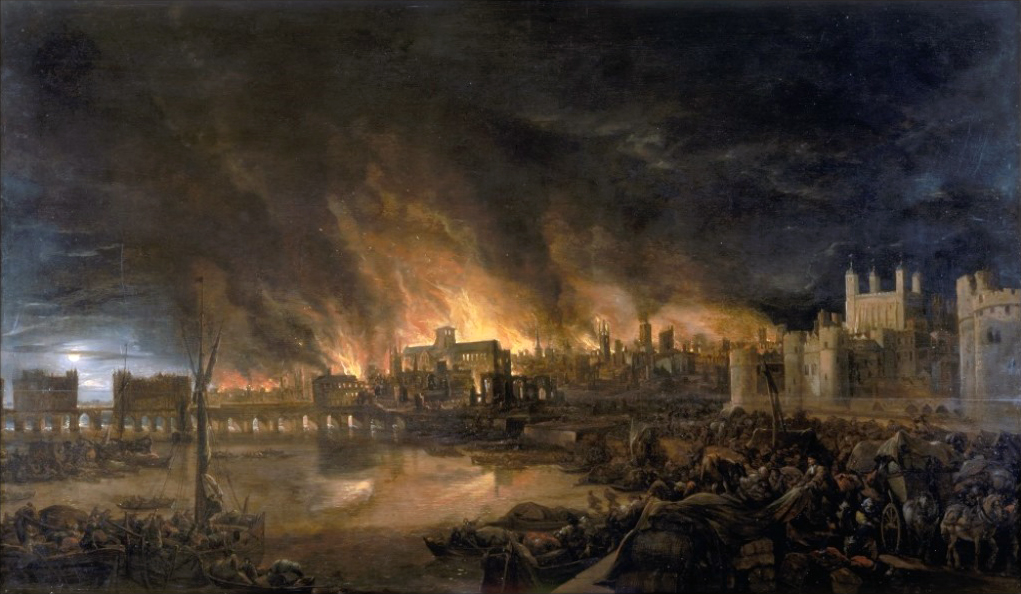
\includegraphics[width=0.8\linewidth]{Plots/london_fire.jpg}
\end{figure}
Modern insurance is traced back to \blue{the Great Fire of London} in 1666 which has destroyed a big part of the city of London. This event has initiated \blue{fire insurance} protection against such disastrous events. 
\end{frame}

\begin{frame}{保险(insurance)}
\begin{itemize}
\item Insurance originates from a general demand of society who asks for protection against \blue{unforeseeable events} which might cause \blue{financial damage} to individuals and society. 
\item The general solution is to build a community to which everybody contributes a \blue{fixed deterministic premium} and then the \blue{unforeseeable financial damage} is financed by the means of this community.
\end{itemize}
\end{frame}

\begin{frame}{保险公司(insurer)和被保险人(insured)}
This community is developed to \blue{insurer}, and the contributors are called \blue{insured} or \blue{policyholders}.
\begin{figure}
\centering
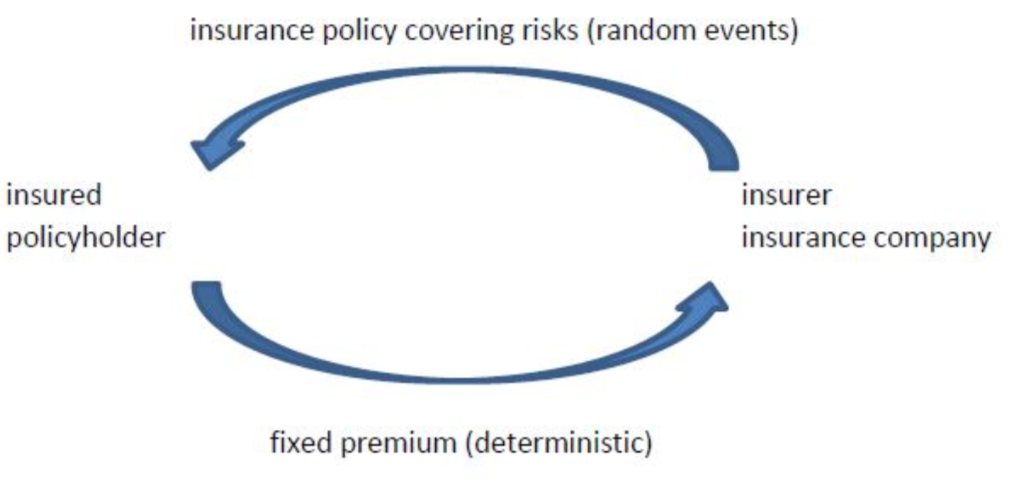
\includegraphics[width=0.8\linewidth]{Plots/insurance.png}
\end{figure}
\end{frame}



\begin{frame}{保险合同(insurance contracts (policies))}
\begin{itemize}
%\item Non-life insurance comprises car insurance, \blue{liability insurance, property insurance}, accident and health insurance, marine insurance, credit insurance, legal protection insurance, travel insurance and other similar products.
\item \blue{Insurance contracts} for these products always specify an \blue{insurance period} (typically of one year). 
\item The \blue{insured events} must occur \blue{within} this insurance period, and cause \blue{financial damage}.
\item The financial damage is \blue{indemnified} by insurer's payment. 
\item Such \blue{random} payments are called \blue{insurance claims}.
\end{itemize}
\end{frame}


\begin{frame}{大数定理(the law of large numbers)}
\begin{itemize}
\item Typically, the insurance \blue{premium} is paid at the \blue{beginning} of the insurance period (upfront). 
\item To determine this insurance premium, the insurance company pools \blue{similar risks} whose individual \blue{insurance claims} can be described by a sequence $Y_1,\ldots, Y_n$ of \blue{random variables}. 
\item These insurance claims $Y_i$ are \blue{random} at the beginning of the insurance period, and therefore need to be described with \blue{probability theory}. 
\end{itemize}
\end{frame}

\begin{frame}{大数定理(the law of large numbers)}
\begin{itemize}
\item Assume $Y_1,\ldots,Y_n$ are \blue{uncorrelated} and \blue{identically} distributed random variables with \blue{finite mean} $\mu = \mathbb{E}[Y_i]$. 
\item \blue{The weak law of large numbers (LLN)} says that for all $\varepsilon>0$
\begin{equation}\label{lln}
\lim_{n\rightarrow \infty} \mathbb{P}\left[\left|\frac{1}{n}\sum_{i=1}^nY_i-\mu \right|\geq\varepsilon  \right]  =0
\end{equation}
\item This means that the \blue{average} claim amount $1/n\sum_{i=1}^nY_i$ becomes more \blue{``predictable''} with increasing \blue{portfolio size} $n$. 
\item Therefore, we can calculate the insurance premium quite \blue{accurately} for \blue{large} portfolio sizes $n$. 
\end{itemize}
\end{frame}

\begin{frame}{伯努利(Bernoulli)}
\begin{figure}
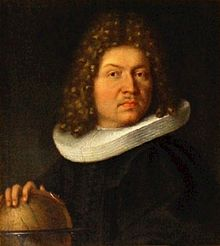
\includegraphics[width=0.3\linewidth]{Plots/Bernoulli.jpg}
\end{figure}
The weak law of large numbers is considered to be a \blue{theoretical cornerstone of insurance}. It goes back to the Swiss mathematician \blue{Jakob Bernoulli} (1655-1705) of the famous Bernoulli family.
\end{frame}

\begin{frame}{中心极限定理(central limit theorem)}
\begin{itemize}
\item For \blue{independent} and \blue{identically} distributed random variables $Y_1, Y_2, \ldots$ with \blue{finite variances} $\sigma^2$, the weak law of large numbers can further be refined by \blue{the central limit theorem (CLT)} which provides the \blue{asymptotic limit distribution}. 
\item The CLT states that we have the following \blue{convergence in distribution}:
\begin{equation}\label{clt}
\frac{\sum_{i=1}^n Y_i-n\mu}{\sqrt{n}\sigma}\rightarrow \mathcal{N}(0,1) \text{~~~as~~~} n\rightarrow\infty
\end{equation}
\end{itemize}
\end{frame}

\begin{frame}{中心极限定理(central limit theorem)}
\begin{itemize}
\item We obtain a \blue{standard Gaussian distribution (normal distribution)}. 
\item The denominator increases of order \blue{$\sqrt{n}$}, a slower rate than $n$. 
\item This implies that the \blue{confidence bounds} of average claims amount get \blue{narrower} with the \blue{larger} portfolio size. 
\item These are the basics why insurance works.
\end{itemize}
\end{frame}

\begin{frame}{高斯(Gauss)}
\begin{figure}
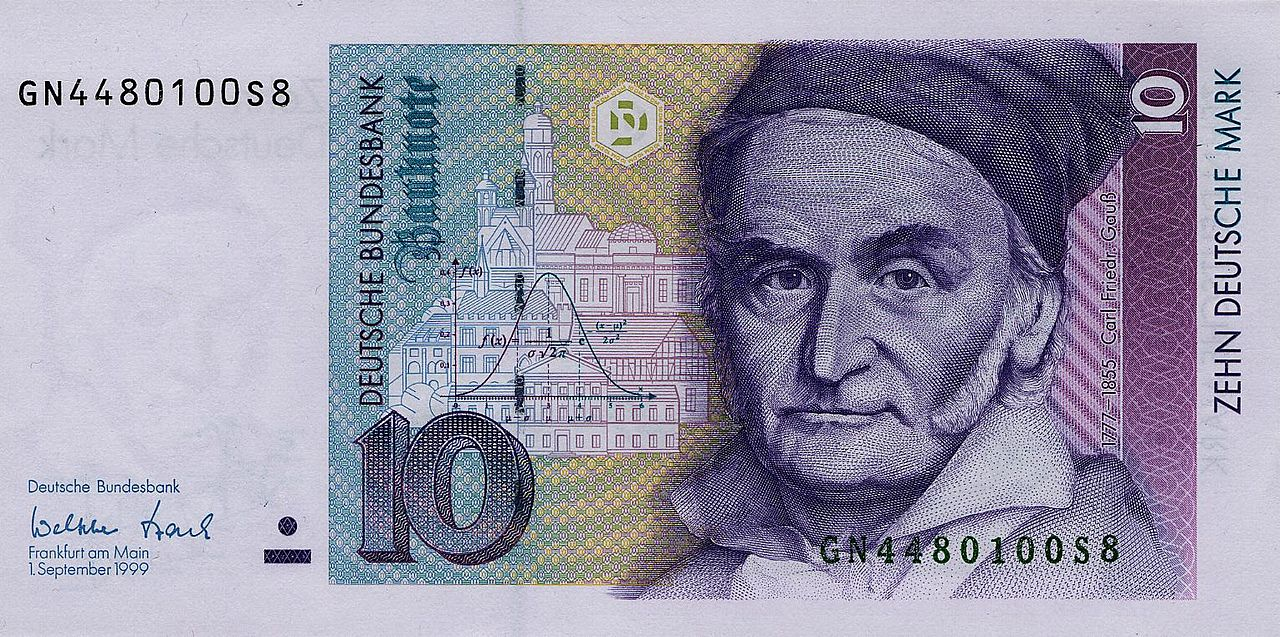
\includegraphics[width=0.7\linewidth]{Plots/Gauss.jpg}
\end{figure}
The \blue{Gaussian distribution (normal distribution)} is named after the German mathematician \blue{Carl Friedrich Gauss} (1777-1855). He was one of the greatest mathematicians and has contributed to many different fields in mathematics and physics. 
\end{frame}


%%normal frame
%\section{非寿险的种类}
\begin{frame}{非寿险的种类}
	\begin{itemize}
		\item \red{财产保险(property insurance)}是以财产及其相关利益为\blue{保险标的},~当保险事故发生导致被保险财产遭受损失时,~由保险人以金钱或实物对被保险人进行补偿的一种保险.如\blue{车损险(body damage),~盗抢险(theft and robbery)}.
		\item \red{责任保险(liability insurance)}以被保险人依法应负的民事损害赔偿责任或经过特别约定的合同责任为保险标的.~其保险责任包括两类:~被保险人应负的经济赔偿责任;~因责任判定赔偿纠纷引起的应由被保险人支付的费用.~如\blue{交强险(compulsory third party, CTP),~第三者责任险(third party liability)}.
		\item \blue{短期健康和意外伤害保险(short-term health insurance, casualty insurance)}.
	\end{itemize}

~

注:~ \red{红色}一般表示最重要的概念,~\blue{蓝色}次之.
\end{frame}
%\section{非寿险和寿险的比较}
\begin{frame}{非寿险和寿险的比较}
	\begin{table}[]
		\centering
		\caption{非寿险(\blue{non-life, general, property\&casualty insurance})与寿险(life insurance)的比较}
		\label{my-label}
		\begin{tabular}{lll}
			\hline
			& 寿险 & 非寿险 \\ \hline
			退保转保 & 业务稳定               & 业务极不稳定                                             \\
			合同期限 & 长期合同               & 短期合同                                               \\
			赔付金额 & 赔付金额具有可预期性         & 赔付金额有很强的随机性                                    \\
			概率依据 & 生命表                & 历史赔付                                               \\ \hline
		\end{tabular}
	\end{table}
\end{frame}
%\section{非寿险精算中的主要数学和统计知识}
\begin{frame}{非寿险精算中的主要数学和统计知识}
	\begin{enumerate}
		\item 集体风险模型(collective risk modelling)			
		\item 个体风险模型(individual risk modelling)
		\item 破产理论(ruin theory)	
		\item \green{费率厘定(pricing)}
		\item \green{贝叶斯模型和信度理论(Bayesian models and credibility theory)}
		\item \green{准备金评估模型(claims reserving)}
		\item \green{机器学习(machine learning)}.~参考资料\cite{WB}.
	\end{enumerate}
	其中4-7点为本课程主要介绍的内容.
	
	~
	
	注:~\green{加粗}一般用来强调或者对比.
\end{frame}

%\section{参考资料}
\begin{frame}{参考资料}

\begin{itemize}
	\item 以下按照\green{优先级}列出.~\cite{no1},\cite{Meng}为必读,~其它为选读.
	\item 选读中, ~\cite{WB}为机器学习内容,~\cite{WB2}涵盖非寿险精算中的大部分知识,~\cite{Friedland}和\cite{Werner}为Casualty Actuarial Society Exam 5的参考资料.
\end{itemize}
\end{frame}

\begin{frame}{参考资料}

~

{\small
	\begin{thebibliography}{99}
		\bibitem{no1}
		本幻灯片
		
		\bibitem{Meng}
		孟生旺,刘乐平,肖争艳,高光远 (2019).
		{\it 非寿险精算学,第四版}.北京:中国人民大学出版社.
		
		%\bibitem{Wu1}
		%W\"uthrich, M.V. (2017).
		%Covariate selection from telematics car driving data.
		%{\it European Actuarial Journal} {\bf 7/1}, 89-108.
		
		
		%\bibitem{Gao}
		%Gao, G., W\"uthrich, M.V. (2017).
		%Feature extraction from telematics car driving heatmaps. Available at SSRN:https://ssrn.com/abstract=3070069.
		
		
		%\bibitem{Gao&Meng}
		%Gao, G., Meng, S., W\"uthrich, M.V. (2018). Claims frequency modeling using telematics car driving data. Available at SSRN: https://ssrn.com/abstract=3102371.
		
		
		
		\bibitem{WB}
		W\"uthrich, M.V., Buser, C. (2019).
		Data analytics for non-life insurance pricing.
		Available at SSRN: https://ssrn.com/abstract=2870308.
		
		\bibitem{WB2}
		W\"uthrich, M.V. (2020). Non-Life Insurance: Mathematics \& Statistics. Available at SSRN: https://ssrn.com/abstract=2319328.
		
		\bibitem{Friedland}
		Friedland, J. (2010). Estimating unpaid claims using basic techniques. 3rd edition. {\it Casualty Actuarial Society study notes}.
		
		\bibitem{Werner}
		Werner, G., Modlin, C. (2016). Basic ratemaking. 5th edition.{\it Casualty Actuarial Society study notes}.
	\end{thebibliography}}
\end{frame}


\end{document}